\documentclass[a4paper,12pt,twoside]{report}
\usepackage[left=2cm,right=2cm,top=2cm,bottom=3cm]{geometry}
%\geometry{a4} 
%\include{preamble}

%% Language and font encodings
%\usepackage[english]{babel}
%\usepackage[utf8x]{inputenc}
%\usepackage[T1]{fontenc}
%% Useful packages
\usepackage{listings}
\usepackage{amsmath}
\usepackage[colorlinks=true, allcolors=blue]{hyperref}

\usepackage{graphicx}
\graphicspath{{images/}}

\usepackage{parskip}
\renewcommand{\baselinestretch}{1.2}

% Title
\title{Applying the polyhedral model to tile loops in Devito}
\author{Dylan McCormick}

% Document
\begin{document}
\maketitle

\tableofcontents

%%% INTRODUCTION %%%
\chapter{Introduction} % Devito!
There are many established optimizations which improve the run-time performance of program loops and have been in use for decades.
The theory of why these optimizations work is has been researched extensively [uniformloop, others] and has been practically applied in modern optimizing compilers so
transformed code need not always be hand-written. Some transformations have a negative effect on the readability and maintainability of code by
increasing code size and changing statement ordering. This can make them undesirable or even infeasible to develop and maintain by hand, in spite
of their performance benefits. It is an attractive option to have a smart compiler or code generator make the transformations automatically so the
original computation description remains concise. Automatically identifying and taking advantage of opportunities for loop optimizations is a tremendous
challenge for an optimizing tool which has to ensure program correctness based on the information available in the source code. If the tool cannot guarantee
correctness or appreciate the logical implications of a piece of code then no transformation occurs, resulting in a potential performance opportunity cost.
Some tools operate in a more domain-specific context where the problems they handle pertain to a particular field; for example, seismic imaging.
Such tools have more knowledge about possible inputs and what requirements applications in the domain have. This allows them to rely on more
assumptions and often apply more aggressive optimizations.

In scientific computing applications code which performs many more floating point operations than memory accesses is common, particularly 
where numerical methods are employed. Such computations often make extensive use of loop nests to iterate over multi-dimensional structures and perform calculations
at each step, such as code which iterates over pairs of matrices to compute their product. The code inside these loops is typically where these computations 
spend most of their time [dragon cite], so there is much to be gained in terms of performance and efficiency by studying improvements and optimizations that 
can be made to this type of code, especially when dealing with real-world large-scale problems like seismic imaging.

Automated code generation is an increasingly important solution to the problem of writing high-performance code
for scientific applications. Decades of research into compiler optimizations and advanced computer architecture developments
have uncovered a number of techniques that can be applied in translating high-level problem descriptions into low-level source code
to achieve some form of performance increase. The complexity of modern systems and computational problems makes it increasingly 
difficult for a software engineer to produce maximally efficient code by hand even with the help of smart
compilers. This is additionally challenging for scientists and researchers whose specialization is not in software engineering. Tools
and frameworks for automatic generation of application-specific high-performance code from high-level or even symbolic input are a very
attractive option for improving performance of numerical computations. Devito is one such tool which generates high-performance code from high-level symbolic
input which approximates partial differential equations typically applied in the seismic imaging domain. It currently applies a number 
of optimizations and analyses [devito cite] when generating code, but could benefit from additional loop optimizations that improve performance for some problems.

% http://dl.acm.org/citation.cfm?id=109108

\section{Loop tiling}
One optimization that can improve the performance of a loop nest is known as `loop tiling' or `loop blocking', which improves data locality and parallelism
by transforming the way a loop nests iterates over its domain. Loop tiling is one of the primary optimizations researched during this project.
Loops which have been tiled can sometimes be further optimized in ways that were previously impossible. For example, 
loop-invariant code motion (LICM) transformations on non-tiled code can be restricted by available memory when 'moving'
statements from within a loop with a high number of iterations. This limitation can be overcome when LICM is applied to tiled code. Such
loop nests and transformations lend themselves well to geometric reasoning as loops can be considered as dimensions in space and time and individual
iterations as integral points within those dimensions. This gives rise to a host of theory and tools (so-called polyhedral tools) which apply polyhedral 
techniques to reason about and optimize loop nests.

\section{Main contributions}
The contributions of this project are as follows;
\begin{itemize}
	\item{Identify an opportunity for loop-tiling optimizations to be applied by Devito}
	\item{Demonstrate performance increase of optimizations applied to automatically-generated loop nests}
	\item{Devise and implement features in Devito which drive polyhedral tools to automate generation of tiled code}
	\item{Analyse performance results produced by new features}
	\item{Increase run-time performance gains realized by Devito users}
\end{itemize}

\chapter{Background}

\section{Fundamentals}
\subsection{Compilers}
A compiler is a piece of software which produces code in a target language by assembling and interpreting input code in a source language.
Typically, compilers are used to translate a high-level programming language which describes computation to a human developer [example] into 
a low-level programming language [example] which is understood by a computer. Due to the complexity of modern languages, systems and computer
architectures this is not a straightforward translation and compilers have a lot of freedom in how they choose to interpret, transform and analyze
their input in order to produce output that meets certain requirements. For example, a compiler might reorder certain instructions from the input
program to produce output code which executes faster than without the instruction reordering.
[Compilation process diagram]

In addition to common `general purpose compilers' (such as \texttt{gcc} or \texttt{javac} which compile C and java programs respectively),
there are `high-level compilers' which don't generate low-level executable code and `domain-specific compilers' which somtimes operate on
custom language inputs and are designed for programs in a particular field.

\subsection{Loops}
A common construct in modern code, especially when implementing numerical methods, is the `loop'. Virtually every program spends most of its 
time executing loops [Dragon 531], so compiler designers who are interested in optimization dedicate much research to 
loop transformations and analyses in an effort to reduce their performance impact. The type of loop dealt with in this project is the
`for loop' which is typically structured as in \ref{fig:forloop}. A `for loop' has a `body' of statements which are repeatedly executed
while the `loop condition' holds. There are no special constraints on the types of statements that can feature in the body of a for loop so it
is possible and indeed very common to have a `for loop' present in the body of another `for loop'. Placement of loops within other loops in such a 
is called `nesting' and gives rise to the `loop nest' construct which refers to a group of nested loops. When a loop nest is structured
such that all of its statements are found in the innermost loop body it is known as a `perfect loop nest'.

\begin{figure}[h]
    \begin{lstlisting}[language=C]
        //Loop header defines bounds and step operation
        for(int i=0; i < LIMIT; i++){
            //Loop body contains code executed at each step
            ...
        }
    \end{lstlisting}
    \caption{The structure of a simple for loop in C}
    \label{fig:forloop}
\end{figure}

\subsection{Iteration spaces}
[Dragon 788]
% http://dl.acm.org/citation.cfm?id=2458526 Split Tiling
When analysing and describing iterative computations, particularly with nested iterative components, it can be useful to consider 
all of the iterations described by the code as points in an 'iteration space'. Each point in an iteration space represents a
particular assignment of values to the loop indices. Iteration spaces provide a geometric description of loop nests which can be
transformed and visualised. By considering connections between points in an iteration space, the order of iteration or 
inter-iteration dependencies can also be described. Iteration spaces are used throughout this paper to explain the research and results obtained.

Take this simple code fragment which iterates over a two-dimensional array and sets its elements to 0
\begin{figure}[h]
    \begin{lstlisting}[language=C]
        int array2d[5][10];

        for(int i=0; i<5; i++){
            for(int j=0; j<10; j++){
                array2d[i][j] = 0;
            }
        }
    \end{lstlisting}
        \caption{
            This is loop nest iterates over a two-dimensional structure and sets all of its elements to 0. It is an example
            of a `perfect loop nest'.
        }
        \label{fig:2dloop}
\end{figure}

Its iteration space is a rectangle of points representing all the combinations of the loop-indices that are within bounds.

\begin{figure}[h]
    \centering
    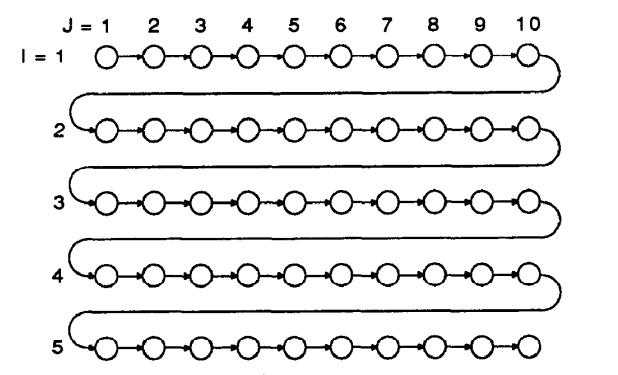
\includegraphics[scale=0.75]{iteration_space}
    \caption{A representation of the iteration space for \ref{fig:2dloop} where arrows indicate the direction of iteration}
    \label{fig:iteration_space}
\end{figure}

A more complex two-dimensional loop nest might perform a computation at each iteration which requires a value from an earlier
computation thereby creating a dependence of on previous iterations. In \ref{fig:2dloop} the computation is trivial and there are no
inter-iteration dependencies since the loop body makes no reference to array elements calculated in earlier iterations.

\begin{figure}[h]
    \begin{lstlisting}[language=C]
        int array2d[100][100];

        for(int i=1; i<100; i++){
            for(int j=1; j<100; j++){
                array2d[i][j] = array2d[i-1][j] 
                              + 2*array2d[i][j-1];
            }
        }
    \end{lstlisting}
    \caption{
        This is loop nest iterates over a two-dimensional structure and updates the value of all but the first elements in each dimension.
        The right hand of the assignment refers to two array indices which were calculated in previous iterations of the \texttt{i} and \texttt{j} loops
        respectively. It is an example of a `perfect loop nest' as well as a `stencil loop'.
    }
    \label{fig:stencil}
\end{figure}

\subsection{Stencils}
% http://dl.acm.org/citation.cfm?id=1413375
A computation which iterates over a grid and performs nearest-neighbour computations is known as a stencil . These are
particularly common when implementing code that deals with numerical methods and partial differential equations.
Each point in the grid is updated some weighted contributions from a subset of its neighbours \cite{stencil}. \ref{fig:stencil} is an example of a stencil.

\subsection{Data locality}
Modern computer architectures have a hierarchy of data caches which store data under locality assumptions that memory locations close to each other
are likely to be used within a short period of time (spatial locality) and that a memory location is likely to be reused (temporal locality). 
When statements in a loop body access a memory location, it is loaded into the data cache hierarchy along with nearby memory locations to pre-empt probable future uses.
However non-optimized loop structures may not make use of this data before it is evicted from the cache by another memory access.
A common goal of loop optimizations is to improve data locality across iterations so that expensive fetches from slower memory can be avoided 
and caching techniques are more efficiently utilised.

\section{Loop optimizations}
Loops have a dominant impact on the performance of most programs that make use of them, particularly if loops are nested.
Most of the time, programmers write loops as succinctly and with as few redundant iterations as possible, making it difficult
for optimizations to truncate iteration spaces while preserving program correctness. Typically, loop optimizations reshape the
way a loop nest traverses its iteration space to try and exploit \textit{data locality} in the underlying computer architecture which
manages the data used by the loop body. There are several common loop optimizations which transform a loop nest structure ie. through
swapping the order of loop headers to exploit data locality, however the primary optimization studied in this project is \textit{loop tiling}.

\subsection{Loop tiling}
\textit{Loop tiling}, also known as \textit{strip mine and interchange} or \textit{loop blocking}\cite{dragon}, is an optimization that modifies 
a loop nest so that it iterates completely over `tiles' or `blocks' of the iteration space, rather than repeatedly iterating 
completely through each dimension of the iteration space until all points are visited. Tiling transformations group points of
the original iteration space into blocks. The resulting blocks have smaller iteration bounds and so the innermost loops are completed more often,
reducing the amount of time before nearby data accesses occur and improving data locality. The tile size can be chosen such that memory locations
required in a full loop execution fit into the cache and prevent excessive eviction. In addition to improving data locality, loop tiling can also 
create opportunities for parallelism not present in the original code.

\subsection{Polyhedral model}
The Polyhedral model is a powerful abstraction for reasoning about loop nests and loop transformations \cite{pluto} that builds on the
geometric representation of loop iterations described in an iteration space. Each iteration of a statement is viewed as an
integral point within a polyhedron that contains all iterations of the statement. With a polyhedron for each statement and an understanding
of the dependencies between statements, linear algebra and linear programming techniques can be applied to transform and scan
the iteration spaces they represent.


%%% CLooG %%%
\section{CLooG}
CLooG (Chunky Loop Generator) is a free software which generates loops that visit each integral
point found within a convex polyhedron in lexicographical order \cite{cloog}. It is also designed to be
the back-end to code generation tools that perform automatic parallelism. Its output is pseudo-code loops which visit
each integral point of a union of polyhedra in such a way as to minimize control overhead and produce efficient code.

\subsection{Motivation}
The polyhedral model allows reasoning about and solving a wide range of problems related to program transformations,
in particular where loop nests are involved. When performing these transformations, code generation is usually the last
step after the abstract structure of the program has been analysed and mutated. There are often constraints on the size of the code
that can be generated to ensure readability for developers and practicality for users attempting to run the code on their machine,
however the most concise code is not always the most efficient, and some transformations may generate complicated loop bounds in an effort
to reduce code size. This type of code can be difficult for a compiler to optimize and for a CPU to schedule in an optimal way due to
poor control management. CLooG provides an interface for applying polyhedral reasoning techniques to generate code which is optimized for control
and within the user's requirements of size or complexity.

We considered CLooG as a candidate for the tiled code generation back-end for Devito because of its simplicity in use and its incorporation into
other tools performing similar tasks as this project's goal. The ability to manually build an input file for a simple example of Devito's
output provided an excellent starting point for understanding how both tools work and for obtaining initial results.

\subsection{Implementation}
CLooG provides a command-line interface which makes use of specially formatted input files (primarily composed of matrices representing
the sets of inequalities defining an iteration space) to understand the loop nest structure as well as a C library that has structures and
functions that permit programmatic configuration and execution of the tool.
Although CLooG is frequently used to make loop-nests parallelizable or more control efficient, it is not concerned with the nature of the
code found within a loop (apart from other loops), and makes no assumptions whatsoever about dependencies between statements.
Statements in CLooG are represented abstractly by inequalities on the iterators which define upon which iterations the statements are executed 
For example the loop body in \ref{fig:stencil} is described to CLooG by its domain, given by the inequalities
\[i \ge 1 , i < 100 , j \ge 1, j < 100 \]

\subsubsection{Algorithm}
The algorithm employed by CLooG for visiting the integral points of the specified polyhedra \cite{polyhedra-algo} is presented in in a simplified form.
For each dimension in the iteration space described by the user input, proceeding from outermost to innermost loops;
\begin{enumerate}
    \item Project the polyhedra onto the corresponding dimension 
    \item Separate the projections into disjoint polyhedra which represent, in this dimension, either the overlapped iteration
        space of multiple statements, or the unique iteration space of a single statement. At this stage, the constraints in the current
        dimension give loop bounds that scan the polyhedra in this dimension. The constraints in the other dimensions are guards on 
        the statements in other dimensions.
    \item Recurse for each polyhedron, projecting in the next dimension.
    \item Sort the resulting loops so that they scan the polyhedra in lexicographical order.
\end{enumerate}
At this stage CLooG has enough information to pretty-print the loops into code.

\subsection{Limitations}
CLooG is a tool usually used as a back-end to a more specialised tool such as PLUTO \cite{pluto} or PrimeTile \cite{primetile} which
apply polyhedral theory to transform a given loop nest to enhance parallelism or data locality and delegate CLooG to generate
efficient code to scan the new polyhedron. CLooG itself however, is not automated in any way and must be driven with a problem
specification that includes inequalities defining the iteration space, and optional `scattering functions' which encode the scheduling
of statements. This makes standalone usage of CLooG somewhat restrictive, but integration into Devito's code generation pipeline
very attractive. An additional technical constraint of CLooG is that it provides a command-line interface and C libraries only,
limiting its ability to interface with other languages such as Python which is common in scientific computing applications.

%%% PLUTO %%%
\section{Pluto}
PLuTo \cite{pluto} is an open-source tool for automatic polyhedral parallelization and locality optimization. Using CLooG as a code generation
back-end, PLuTo applies analytical model-driven transformations in the polyhedral model \cite{ram-polyhedral} to improve the performance
of regular programs containing loop nests. One of the primary features of PLuTo is its automatic exploration of the space
of potential program transformations to identify and apply the most effective loop tiling.

\subsection{Motivation}
Like CLooG, PLuTo is motivated by the powerful abstraction provided by the Polyhedral model when reasoning about and optimizing loop
nests. However PLuTo is more specifically concerned with how loop tiling can improve parallelism and data locality, especially
for applications run on massively parallel architectures like those frequently seen in scientific computing applications. The framework
takes a step further yet by applying analytical methods to intelligently find optimal transformations and tilings with code dependencies in mind.
The tool's design is indicative of its intended usage in optimizing existing code, possibly developed before a tool as capable as PLuTo was developed.

\subsection{Implementation}
PLuTo operates as a source-to-source optimization tool, taking as input a sequence of nested loops in source-code format
and producing a transformed sequences of loops in source code. The research and behind PLuTo is on automated transformations,
not dependence analysis or source-code parsing, so it delegates the task of interpreting input and determining dependencies
to another tool in the polyhedral space, LooPo. The transformation framework implemented in PLuTo takes polyhedral domains representing the iteration
spaces of the original program, as well as dependence polyhedra which encode the dependence structure of the input source-code.

The transformation framework within PLuTo makes use of a bounding cost function to reason about dependences and iteration domains
geometrically and to provide a target to minimise when identifying optimal transformations. The cost function can be formulated
as a system of Integer Linear Programming (ILP) problems which encode legality and cost constraints and can be solved by the Simplex
algorithm. The framework iteratively augments and solves ILP problems to find multiple independent solutions for each statement. With
these solutions, PLuTo is able to construct matrices representing the transformed domains and statement dependencies which can be
given as input to CLooG for code generation.

\subsection{Limitations}
PLuTo is a powerful tool that makes many informed analyses to drive its automated search for optimal transformations, and its integration
with other polyhedral tools make it a well-documented practical tool for users looking to apply source-to-source loop transformations. It
delivers a more specialised, automated solution than using CLooG alone, and allows with existing code to perform optimizations without having to 
analyse the loop and dependence structure of their program. However
PLuTo's generality and source-to-source nature make it unsuitable for direct application in the Devito pipeline. With the specific structure and
nature of code generated by Devito, assumptions can be made that greatly reduce the work a tool like PLuTo would need to do in determining
dependencies and optimal transformations, but the general approach PLuTo takes prevents these assumptions from being made. The source-code level
is also a low-level representation that restricts what can be done by Devito after the transformations take place and would require premature
generation of source code to feed as input to PLuTo.

%%% Devito %%%
\chapter{Devito}
Devito \cite{devito-fd}, \cite{devito-dsl}, is a domain-specific language (DSL) and code generation framework that produces highly-optimised
code for finite-difference computations \cite{opesci-fd}. It uses high-level symbolic problem descriptions that can be hand-written to automatically
generate and optimise high-performance parallel C code for a range of computer architectures. The finite-difference kernels that
Devito generates are used to solve partial differential equations that are primarily used for simulations typical in the oil and gas industry.
% https://arxiv.org/pdf/1605.06381.pdf

\section{Motivation}
Modern high-performance computing applications need to make use of the latest developments in computer architecture to produce truly
powerful solutions. As modern technologies become more powerful they also become more complex with massively parallel systems like
GPGPU (General Purpose Graphics Processing Unit) and advanced architectural capabilities such as vectorization providing opportunities
to improve program performance at the cost of increased implementation complexity. For scientists looking to leverage performant
technologies in their programs the Python programming language is a common choice because of its natural form of expression,
large collection of open-source packages that allow interaction with some of these advanced architectures and its ease of use when compared with traditional languages like C.
However, as an interpreted language Python is not suited for direct use in HPC applications, and currently available methods that reduce the interpreter overhead introduce
additional complexity and are still not as efficient as straight C code. 

Devito aims to combine the ease and expressiveness of Python, with the 
power and optimizations available to C code. By using a domain-specific language embedded in a python package, Devito can provide a specialized interface
that describes numerical computations and perform code generation with aggressive optimizations to produce faster programs that require less HPC expertise
from the developer.

\section{Design}
The high-level architecture of Devito can be broken into four steps;
\begin{enumerate}
    \item Create Devito data objects which associate SymPy function symbols with user data
    \item Build symbolic stencil equations using the created data objects
    \item Build Devito Operator object using symbolic equations
    \item Instruct the Devito Operator to generate low-level optimized code applied to user data
    \item Compile using user-defined compiler settings
\end{enumerate}

\begin{figure}[h]
    \begin{lstlisting}[language=Python]
    from devito import TimeData, Operator
    from sympy.abc import s, h
    # Function symbol associated with user data
    u = TimeData(name=’u’, shape=(nx, ny),
                 time_order=1, space_order=2)
    u.data[0, :] = ui[:]

    # Symbolic equation
    eqn = Eq(u.dt, a * (u.dx2 + u.dy2))
    # Expand finite-difference stencils
    stencil = solve(eqn, u.forward)[0]

    # Devito operator that transforms stencils into array accesses
    op = Operator(stencils=Eq(u.forward, stencil),
                  subs={h: dx, s: dt}, nt=timesteps)

    # Generate low-level code applied to data with Propagator
    op.apply()
    \end{lstlisting}
    \caption{ Setup code for generating a Diffusion kernel in Devito \cite{devitoi-dsl}
    \label{fig:diffusion_devito}
\end{figure}

One of the key benefits of using Devito is the automatic generation of abstract array accesses upon creation of the Operator object. This 
creates an intermediate representation (IR) of the stencil which is then optimized and translated into C when triggered by the user using the Operator
in a process called 'propagation'. It is during this propagation stage that loops are generated, and so this is the point in the process where
Devito will analyse the IR and delegate to CLooG to tile the structure being generated. The objects that make up the IR allow
Devito to programmatically reason about the loop and dependence structure of the kernel which will form the primary input for CLooG's transformation.

\begin{figure}[h]
    \begin{lstlisting}[language=C]
      extern ‘‘C’’ int Operator(float *u_vec)
      {
          float (*u)[1000][1000] = (float (*)[1000][1000]) u_vec;
          {
              int t0;
              int t1;
              #pragma omp parallel
              for (int i3 = 0; i3<500; i3+=1)
              {
                  #pragma omp single
                  {
                      t0 = (i3)%(2);
                      t1 = (t0 + 1)%(2);

                  }
                  {
                      #pragma omp for schedule(static)
                      for (int i1 = 1; i1<999; i1++)
                      {
                          #pragma omp simd aligned(u:64)
                          for (int i2 = 1; i2<999; i2++)
                          {
                              u[t1][i1][i2] = 2.5e-1F*u[t0][i1][i2-1]
                                            + 2.5e-1F*u[t0][i1][i2+1]
                                            + 2.5e-1F*u[t0][i1-1][i2]
                                            + 2.5e-1F*u[t0][i1+1][i2];

                          }

                      }

                  }

              }

          }
      }
    \end{lstlisting}
    \caption{Auto-generated C code to solve the diffusion example in \ref{fig:diffusion_devito} \cite{dsl}}
    \label{fig:diffusion_C}
\end{figure}

Devito takes its form as a Python library that provides an API for users to create and manage objects that define and configure all of the components
in the code generation pipeline. To make the most of the native Python environment and the practical benefits it brings, Devito does not define its 
own high-level DSL in the traditional sense, instead it makes use of and extends the powerful SymPy Python library for symbolic mathematics. 
The familiar abstraction provided by a native python library allows users to separate implementation and optimization concerns from the numerical computation at hand.

%%% PROJECT PLAN - Pathway to success %%%
\chapter{Project Plan}
Need Timeline!
\begin{itemize}
    \item Research polyhedral transformation and code generation tools
        \begin{itemize}
            \item This step is currently on-going. Having researched and experimented with the tools mentioned in
                this report, we have identified CLooG as a good starting point for performing the experiments needed
                to evaluate our plan.
        \end{itemize}
    \item Manually drive a tool to produce time-tiled code from a simple Devito-generated kernel
        \begin{itemize}
            \item Configuring and running CLooG at this stage has been an exercise in better understanding the polyhedral model,
                loop tiling and the code-generation interface CLooG provides. At present, we have successfully created a basic input file
                which describes a simple Devito kernel and run CLooG with it, however additional input constraints need to be understood and implemented
                before the output from these runs is interesting.
            \item To put Devito ke
                which strip-mines the outer time loop in preparation for the tiling body transformations we intend for CLooG to make. This step was required as CLooG
                transformations cannot add extra dimensionality to a loop nest.
        \end{itemize}
    \item Perform performance experiments on tiled code produced by CLooG.
        \begin{itemize}
            \item With correctly tiled loop nests generated by manually-configured CLooG runs, we can run the code and compare its performance with an equivalent 
                non-tiled kernel. This will give an idea of how well the tool has been configured and what kind of performance gain we should expect to see when
                time-tiling is fully implemented.
        \end{itemize}
    \item Research implementation specifics to devise a workflow for driving CLooG automatically with Devito and feeding the tiled output back into the Devito pipeline.
    \item Implement CLooG as a back-end for automatic tiled code generation in Devito.
    \item Evaluate performance change in tiled Devito-generated kernels compared to non-tiled equivalents.
    \item If the transformations are successful in the way we expect, investigate the extent to which the transformations enable previously infeasible LICM transformations
        in Devito kernels and evaluate the performance benefit for any such LICM optimizations.
    \item Finalize implementation details and experiment results.
    \item Produce final write-up and presentation of results.
\end{itemize}

\chapter{Evaluation Plan}
This project specifically aims to improve performance of code generated by Devito, and evaluating the benefit of the changes made
as a result of research and experiments is crucial to determining the success of the project. Based on an understanding of the theory
behind loop transformations and of the behaviour of Devito kernels, there is an intuitive expectation that time-tiling in Devito will 
have a measurable improvement on kernel run time.
\begin{itemize}
    \item Once tiled code has been generated by CLooG with manual configuration experiments can begin on the performance
        of the tiled code. To determine the impact of the program transformations, the non-tiled and tiled code should be independently
        and sequentially executed on hardware similar to that on which Devito kernels are usually run. Technical considerations must be made
        to minimise the influence of external factors (e.g. Operating System actions or other running processes) and provide a controlled testing
        environment. Multiple Devito kernels should be tested in this way and preference should be given to kernels with high iteration counts
        so that differences in execution time are more pronounced. Based on the results obtained at this stage, changes can be made to the configuration
        of CLooG as corrections or experiments with different tiling parameters. If the results indicate performance improvements then the project can advance
        to the implementation stage.
    \item Performance experiments will be focussed on kernels for two fundamental problems in the oil and gas industry; namely the acoustic wave kernels
        and tilted transverse isotropy (TTI) kernels (Devito gihub cite) which are alread well-research in the Devito framework. The mathematics 
        behind these two problems produces quite different kernels with contrasting levels of complexity.
        \begin{itemize}
            \item \textbf{Acoustic wave equation:} Wave equations are linked to many physical phenomena (TJ cite) and the acoustic wave equation (AWE) describes the propagation
                of acoustic waves through a medium. AWE kernels typically have few operations in the main loop body which update grid points over time based on
                the values at other grid points that are nearby in both space and time. The code in \ref{fig:acoustic} is an example of the main loop kernel for the AWE 
                in one dimension. The relative simplicity of this problem makes it suitable for manually-configured experiments as well as being a good exercise 
                in understanding what transformations CLooG can perform and how to drive it to produce them.
            \item \textbf{Tilted Transverse Isotropy:} The TTI problem is similar to the AWE as it also models wave propagation but is more complex in that it can be
                applied to stratified media (such as those found naturally in the earth) and handles propagations which are at an angle with the vertical axis. This
                type of model more realistic than the AWE and very applicable in seismic imaging applications. Kernels which perform TTI computations
                have significantly more statements in the main loop body than AWE kernels and make use of trigonometric operations in addition to floating point 
                arithmetic. Consequently, TTI kernels have a very high arithmetic intensity and it is possible they will see a less marked improvement as a result
                of loop tiling when compared to the AWE kernel.
        \end{itemize}
    \item Before implementation can fully begin, it is important that the design chosen to implement a code generation back-end to Devito be considered carefully.
        CLooG does not provide a native Python API and so with a project timescale in mind, a plausible implementation plan should be made once adequate results s.
    \item After the implementation stage, tests should be performed to ensure the numerical correctness of generated kernels and that transformations are
        being applied as expected.
    \item If no implementation bugs remain, performance testing can begin once again. With support in Devito for automated tiled-loop generation, evaluation at this
        stage should proceed in a large scale automated fashion. A set of problem descriptions that represent the different types of kernel Devito can produce is
        important to ensure that performance changes are understood across all applications of Devito. In particular, if for any reason a kernel experiences a slowdown
        then additional experiments must be performed to determine if the code can benefit from being transformed and if not, changes must be made in Devito to make sure
        it never generates sub-optimal code.
    \item When evaluating performance, several metrics should be considered;
        \begin{itemize}
            \item Devito run time when generating transformed programs
            \item Overall kernel run time
            \item Floating point operations per second (FLOPS)
            \item Cache performance (misses, hits)
            \item Compilation time and compiled size
            \item Memory usage
        \end{itemize}
    \item The primary criterion for success is decreased running time of Devito kernels, and this improvement should follow from improved cache performance 
        (fewer misses) and increased FLOPS.
    \item Since Devito is a user-facing tool, feedback should also be obtained regarding the applicability and usability of the new features.
\end{itemize}

\begin{figure}[h]
    \begin{lstlisting}[language=C]
        for(int t=1; t<T; t++){ //time loop
            for(int i=1; i<N; i++){ //1D space loop
                u[i][n+1] = 2*u[i][n] - u[i][n-1] - pow(C, 2.0)*(u[i+1][n]
                          - 2*u[i][n] + u[i-1][n]);
            }
        }
    \end{lstlisting}
    \caption{
        A simplified presentation of the main loop for an acoustic wave equation kernel in 1D (TJ cite). Here a point grid \texttt{u} at time
        \texttt{n+1} is calculated by a weighted combination of nearby points \texttt{i+1} and \texttt{i-1} in the previous two timesteps \texttt{n} and \texttt{n-1}
		\cite{opesci-fd}
    }
    \label{fig:acoustic}
\end{figure}

\section{Risks}
Even with the domain-specific context in which Devito operates, the problems for which it generates code can vary significantly in their practical application
as well as their implementation. The theory of how loop tiling can improve performance is understood, but that does not mean tiled code which experiences better
data locality that non tiled code results in better program run time. There are other potential bottlenecks during program execution which could be the dominating
restrictions on execution time for certain kernels, preventing the tiling transformations from having a noticeable improvement.

\subsection{Arithmetic Intensity}
Arithmetic intensity is the ratio of FLOPS per byte of memory traffic and indicates how memory-bound or computationally-bound a given program is.
Some Devito kernels (such as one implementing an acoustic wave equation) have a small number of statements in their innermost loop, which typically
implies that upon each iteration a small number of floating point operations are performed to update a small area of the grid. Other kernels derived from different 
equations might have many hundreds of statements in their innermost loop, so at each iteration many statements perform local floating point operations before updating
a small section of the grid. The arithmetic intensity for the latter type of kernels can be significantly higher than for the former, and for such programs
we might expect loop tiling to have limited performance benefit since the computational power of the executing system is already being pushed near its limit. This makes
the initial experiments particularly important as they should allow us to identify to what extent the tiling transformations will impact the different types of kernel
Devito can generate.

\subsection{Architecture}
The benefits realized by tiling loops to improve data locality are highly dependent on the architecture of the system upon which the code is executed. Tiling parameters
effect the size and shape of the memory space that is accessed by a loop nest, and an optimal tiling transformation will configure the iteration space such that it both
properly fits and makes the most use of the architecture's underlying memory hierarchy. When designing and testing tiling configurations care must be taken that
relevant architectures are considered and that parameters are chosen which best suit the executing system.

%%% CITATIONS %%%
\chapter{Citations}
\bibliographystyle{alpha}
\bibliography{sample}

\end{document}
